% Options for packages loaded elsewhere
\PassOptionsToPackage{unicode}{hyperref}
\PassOptionsToPackage{hyphens}{url}
%
\documentclass[
  man,floatsintext]{apa6}
\usepackage{amsmath,amssymb}
\usepackage{iftex}
\ifPDFTeX
  \usepackage[T1]{fontenc}
  \usepackage[utf8]{inputenc}
  \usepackage{textcomp} % provide euro and other symbols
\else % if luatex or xetex
  \usepackage{unicode-math} % this also loads fontspec
  \defaultfontfeatures{Scale=MatchLowercase}
  \defaultfontfeatures[\rmfamily]{Ligatures=TeX,Scale=1}
\fi
\usepackage{lmodern}
\ifPDFTeX\else
  % xetex/luatex font selection
\fi
% Use upquote if available, for straight quotes in verbatim environments
\IfFileExists{upquote.sty}{\usepackage{upquote}}{}
\IfFileExists{microtype.sty}{% use microtype if available
  \usepackage[]{microtype}
  \UseMicrotypeSet[protrusion]{basicmath} % disable protrusion for tt fonts
}{}
\makeatletter
\@ifundefined{KOMAClassName}{% if non-KOMA class
  \IfFileExists{parskip.sty}{%
    \usepackage{parskip}
  }{% else
    \setlength{\parindent}{0pt}
    \setlength{\parskip}{6pt plus 2pt minus 1pt}}
}{% if KOMA class
  \KOMAoptions{parskip=half}}
\makeatother
\usepackage{xcolor}
\usepackage{graphicx}
\makeatletter
\def\maxwidth{\ifdim\Gin@nat@width>\linewidth\linewidth\else\Gin@nat@width\fi}
\def\maxheight{\ifdim\Gin@nat@height>\textheight\textheight\else\Gin@nat@height\fi}
\makeatother
% Scale images if necessary, so that they will not overflow the page
% margins by default, and it is still possible to overwrite the defaults
% using explicit options in \includegraphics[width, height, ...]{}
\setkeys{Gin}{width=\maxwidth,height=\maxheight,keepaspectratio}
% Set default figure placement to htbp
\makeatletter
\def\fps@figure{htbp}
\makeatother
\setlength{\emergencystretch}{3em} % prevent overfull lines
\providecommand{\tightlist}{%
  \setlength{\itemsep}{0pt}\setlength{\parskip}{0pt}}
\setcounter{secnumdepth}{-\maxdimen} % remove section numbering
% Make \paragraph and \subparagraph free-standing
\ifx\paragraph\undefined\else
  \let\oldparagraph\paragraph
  \renewcommand{\paragraph}[1]{\oldparagraph{#1}\mbox{}}
\fi
\ifx\subparagraph\undefined\else
  \let\oldsubparagraph\subparagraph
  \renewcommand{\subparagraph}[1]{\oldsubparagraph{#1}\mbox{}}
\fi
\newlength{\cslhangindent}
\setlength{\cslhangindent}{1.5em}
\newlength{\csllabelwidth}
\setlength{\csllabelwidth}{3em}
\newlength{\cslentryspacingunit} % times entry-spacing
\setlength{\cslentryspacingunit}{\parskip}
\newenvironment{CSLReferences}[2] % #1 hanging-ident, #2 entry spacing
 {% don't indent paragraphs
  \setlength{\parindent}{0pt}
  % turn on hanging indent if param 1 is 1
  \ifodd #1
  \let\oldpar\par
  \def\par{\hangindent=\cslhangindent\oldpar}
  \fi
  % set entry spacing
  \setlength{\parskip}{#2\cslentryspacingunit}
 }%
 {}
\usepackage{calc}
\newcommand{\CSLBlock}[1]{#1\hfill\break}
\newcommand{\CSLLeftMargin}[1]{\parbox[t]{\csllabelwidth}{#1}}
\newcommand{\CSLRightInline}[1]{\parbox[t]{\linewidth - \csllabelwidth}{#1}\break}
\newcommand{\CSLIndent}[1]{\hspace{\cslhangindent}#1}
\ifLuaTeX
\usepackage[bidi=basic]{babel}
\else
\usepackage[bidi=default]{babel}
\fi
\babelprovide[main,import]{english}
% get rid of language-specific shorthands (see #6817):
\let\LanguageShortHands\languageshorthands
\def\languageshorthands#1{}
% Manuscript styling
\usepackage{upgreek}
\captionsetup{font=singlespacing,justification=justified}

% Table formatting
\usepackage{longtable}
\usepackage{lscape}
% \usepackage[counterclockwise]{rotating}   % Landscape page setup for large tables
\usepackage{multirow}		% Table styling
\usepackage{tabularx}		% Control Column width
\usepackage[flushleft]{threeparttable}	% Allows for three part tables with a specified notes section
\usepackage{threeparttablex}            % Lets threeparttable work with longtable

% Create new environments so endfloat can handle them
% \newenvironment{ltable}
%   {\begin{landscape}\centering\begin{threeparttable}}
%   {\end{threeparttable}\end{landscape}}
\newenvironment{lltable}{\begin{landscape}\centering\begin{ThreePartTable}}{\end{ThreePartTable}\end{landscape}}

% Enables adjusting longtable caption width to table width
% Solution found at http://golatex.de/longtable-mit-caption-so-breit-wie-die-tabelle-t15767.html
\makeatletter
\newcommand\LastLTentrywidth{1em}
\newlength\longtablewidth
\setlength{\longtablewidth}{1in}
\newcommand{\getlongtablewidth}{\begingroup \ifcsname LT@\roman{LT@tables}\endcsname \global\longtablewidth=0pt \renewcommand{\LT@entry}[2]{\global\advance\longtablewidth by ##2\relax\gdef\LastLTentrywidth{##2}}\@nameuse{LT@\roman{LT@tables}} \fi \endgroup}

% \setlength{\parindent}{0.5in}
% \setlength{\parskip}{0pt plus 0pt minus 0pt}

% Overwrite redefinition of paragraph and subparagraph by the default LaTeX template
% See https://github.com/crsh/papaja/issues/292
\makeatletter
\renewcommand{\paragraph}{\@startsection{paragraph}{4}{\parindent}%
  {0\baselineskip \@plus 0.2ex \@minus 0.2ex}%
  {-1em}%
  {\normalfont\normalsize\bfseries\itshape\typesectitle}}

\renewcommand{\subparagraph}[1]{\@startsection{subparagraph}{5}{1em}%
  {0\baselineskip \@plus 0.2ex \@minus 0.2ex}%
  {-\z@\relax}%
  {\normalfont\normalsize\itshape\hspace{\parindent}{#1}\textit{\addperi}}{\relax}}
\makeatother

\makeatletter
\usepackage{etoolbox}
\patchcmd{\maketitle}
  {\section{\normalfont\normalsize\abstractname}}
  {\section*{\normalfont\normalsize\abstractname}}
  {}{\typeout{Failed to patch abstract.}}
\patchcmd{\maketitle}
  {\section{\protect\normalfont{\@title}}}
  {\section*{\protect\normalfont{\@title}}}
  {}{\typeout{Failed to patch title.}}
\makeatother

\usepackage{xpatch}
\makeatletter
\xapptocmd\appendix
  {\xapptocmd\section
    {\addcontentsline{toc}{section}{\appendixname\ifoneappendix\else~\theappendix\fi\\: #1}}
    {}{\InnerPatchFailed}%
  }
{}{\PatchFailed}
\keywords{Gender difference, Advice, Interpresonal relationship\newline\indent Word count: 4,362}
\usepackage{csquotes}
\usepackage{setspace, appendix, placeins, booktabs, tikz, siunitx}
\usepackage{tabularx, epigraph, float, colortbl, tabu, pdflscape}
\usetikzlibrary{positioning}
\raggedbottom
\usepackage[maxfloats=256]{morefloats}
\maxdeadcycles=1000
\ifLuaTeX
  \usepackage{selnolig}  % disable illegal ligatures
\fi
\IfFileExists{bookmark.sty}{\usepackage{bookmark}}{\usepackage{hyperref}}
\IfFileExists{xurl.sty}{\usepackage{xurl}}{} % add URL line breaks if available
\urlstyle{same}
\hypersetup{
  pdftitle={Flattering Advice: Avoiding Disappointment as a Driver of Gender Discrimination},
  pdfauthor={Amanda Chen1 \& David Hagmann1},
  pdflang={en-EN},
  pdfkeywords={Gender difference, Advice, Interpresonal relationship},
  hidelinks,
  pdfcreator={LaTeX via pandoc}}

\title{Flattering Advice: Avoiding Disappointment as a Driver of Gender Discrimination}
\author{Amanda Chen\textsuperscript{1} \& David Hagmann\textsuperscript{1}}
\date{}


\shorttitle{Flattering Advice}

\authornote{

The authors are grateful to a lot of things.

Correspondence concerning this article should be addressed to Amanda Chen, Department of Management, The Hong Kong University of Science and Technology, Hong Kong. E-mail: \href{mailto:zchengj@connect.ust.hk}{\nolinkurl{zchengj@connect.ust.hk}}

}

\affiliation{\vspace{0.5cm}\textsuperscript{1} The Hong Kong University of Science and Technology}

\note{

8 January, 2024

}

\abstract{%
This is an interesting project! Please read through it!
}



\begin{document}
\maketitle

\hypertarget{introduction}{%
\section{Introduction}\label{introduction}}

Seeking and giving advice can be challenging conversations to navigate. Advice seekers may be embarrassed to ask for help (Bénabou, Jaroszewicz, \& Loewenstein, 2022), and they may fail to do so if the information they receive could lead to disappointment (Gill \& Prowse, 2012). Indeed, people prefer advisers who withhold unpleasant information (Shalvi, Soraperra, Weele, \& Villeval, 2019) and punish those who tell them things they do not want to hear (John, Jeong, Gino, \& Huang, 2019). People appear to engage in strategic selection of advice to avoid unpleasant information and protect the utility they get from positive beliefs about themselves and the future they anticipate (Loewenstein, 1987; Loewenstein \& Molnar, 2018). But do advice givers anticipate and consider the hedonic cost of honest information to the recipient? While previous work has emphasized the instrumental value of advice (e.g., satisfaction with a decision or accuracy of a prediction), we focus on the motivations of the person providing advice.

Research on advice has largely focused on settings that do not tackle belief utility. For example, participants may have been asked to estimate the number of balls in an urn or choose from pairs of lotteries (Benjamin \& Budescu, 2015). Advisers have been shown to be motivated to give accurate advice (Jonas \& Frey, 2003), and engage in perspective-taking to meet the preferences of the advisee (L. J. Kray, 2000; L. Kray \& Gonzalez, 1999). When they are uncertain, they prefer that advisees do not rely (extensively) on their recommendations (Ache, Rader, \& Hütter, 2020). Thus, it seems that people are concerned about providing good advice even when they are not incentivized for the recipient's decision quality.

In many real settings, however, advice incorporates beliefs about the recipient. Someone recommending an expensive restaurant conveys that they think the advisee is wealthy enough to afford an expensive meal, and someone recommending a student pursue a PhD in economics assumes that they are intellectually capable. Conversely, telling a poorly performing student to switch to a less-demanding major conveys a belief that the student is not capable of improving. Thus, the painful truth may prevent someone from making a bad decision, it may come at a cost to the recipient and damage the relationship between the adviser and advisee. We propose that advisers take these costs into account, even when the interactions are entirely anonymous and they are incentivized for the quality of the advisee's decision.

Specifically, we focus on the signaling value of advice: what does the advice imply about the adviser's perception of the advisee? We propose that advisees have expectations about the advice they receive and treat this as a reference point (Kőszegi \& Rabin, 2006). Advice that falls short of these expectations creates disappointment, while advice that exceeds them is flattering and creates positive interpersonal benefits because it creates a perception that the adviser holds the advisee in high esteem. Such interpersonal considerations may be as important, if not more important, to the adviser than the instrumental value of the advice: the adviser directly experiences a souring relationship, but may suffer little and only much delayed consequences if an advisee makes a poor life decision.

Our account therefore predicts that people receive advice that is more flattering and suggestive of inflated ability and optimistic outcomes than would advice in the absence of such interpersonal considerations. However, we propose that this is not true for all advisees equally. Presenting flattering advice requires the formation of beliefs about the advisee's expectations (reference point). Exley and Nielsen (2022) show that men are more overconfident than women, conditional on equal performance and that people anticipate but fail to incorporate this difference into their decisions. An adviser who seeks to avoid disappointment and incorporates expectations into their advice would then present more favorable advice to male advisees than to female advisees (see Figure 1 for an illustration). This provides a novel account for a well-known finding that men receive more aspirational advice than do women (Kanze, Huang, Conley, \& Higgins, 2018).

Notably, when it pays to have accurate beliefs, such flattering advice would come at a cost: while men would be more likely to aim higher, they would also suffer greater costs from aiming too high and failing to meet the objective. This may seem at odds with a gender gap favoring men. However, observational data often miss people who were unsuccessful. For example, job candidates who ask for a high starting salary may be less likely to receive a job offer, but will also have a higher starting salary conditional on receiving an offer.

In a large, preregistered experiment (n = 2,000), we show that advisers consider the expectations of advisees, even when such expectations do not provide informative insights for the underlying decision-making problem. We find that as a result, showing expectations (but not gender) to advisers leads men to receive more aspirational advice than women. Incorporating expectations leads to worse advice, even when advisers are incentivized based on the outcome of the advisee's decision. In a second preregistered experiment (n = 700), we show that advisers respond to interpersonal considerations. They advice people that they are more attractive than they believe them to be, and inflate to a greater extent when incentivized for likability rather than accuracy. Advisees indeed reward such flattering advice, finding the advisers more likeable and no less trustworthy than those who provide more accurate advice.

\hypertarget{open-science-statement}{%
\section{Open Science Statement}\label{open-science-statement}}

We report all sample sizes, data exclusions, all manipulations, and all measures in the studies. Screen captures of the experimental materials are available in the Supplemental Information. The complete data, code to reproduce all statistical analyses and figures in the manuscript, as well as the preregistration reports are available via OSF. All our studies were preregistered on AsPredicted.org. (will do this later)

\hypertarget{study-1}{%
\section{Study 1}\label{study-1}}

We begin by examining whether advisers take the expectations of advisees into account, even when those expectations are not relevant to the quality of advice. In a three-stage experiment, we first recruit a sample of advisees and ask them to complete a mathematics quiz. After answering all ten multiple-choice questions, participants are anchored to low or high performance expectations and asked to guess how many questions they answered correctly. Next, we recruit advice givers and show them either only the true performance of the advisee, or the true performance and how many questions they guessed they answered correctly. Advisers are tasked with recommending whether the advisee should compete against a group of high-performers or a group of low-performers on the mathematics quiz. Finally, we invite the advisees back and show them the advice they have received. Advisees then pick whether to compete against high or low performers, based on their past performance on the quiz. Our key hypothesis is that advisees who were anchored to high expectations would be more likely to receive advice to compete against the high performer group.

\hypertarget{methods}{%
\subsection{Methods}\label{methods}}

We first recruited a sample of 50 participants from Prolific to complete a 10-question multiple choice mathematics quiz. The questions were taken from a paper-version of the ASVAB standardized exam, such that answers were not available online. Participants had 5 minutes to answer the quiz and were paid 10 cents for each correctly answered question. We define the top 20 scorers as the ``High Performers'' and the bottom 20 scorers as the ``Low Performers.'' On average, participants answered 4.42 questions correctly, High Performers scored between 5 and 10, and Low Performers scored between 0 and 3. We further simulated 1,000 pairings of groups of five participants, with the 5 th percentile of groups scoring an average of 2.60 and the 95 th percentile scoring an average of 6.40. We use these participants as the competitors for the advisees in our main experiment, and the average group scores to anchor expectations.

Next, we recruited 1,002 participants in Stage 1 of our main experiment, for the role of advisees. To arrive at a gender-balanced sample, we dropped the last two male participants to complete the survey, ending up with a sample of 500 men and 500 women (\(M_{\text{Age}}\) = 42.16,50\% Female). Participants completed the same 10-item mathematics quiz as the earlier participants and were informed that their performance would affect their bonus earnings in a follow-up study to be conducted a few days later. After completing the quiz, we informed them of the average score of a group of five participants from the preliminary survey. We randomly assigned them to learn about the 5 th percentile of groups, which scored 2.60. (``Low Expectations'' treatment) or the 95 th percentile of groups, which scored 6.40 (``High Expectations'' treatment). Participants then made a guess (unincentivized) about how many questions they think they answered correctly. The survey concluded with basic demographic questions.

We then recruited 1,000 participants for Stage 2, placing them in the role of advisers. We began by informing them of the mathematics quiz that participants in the preliminary study and Stage 1 had completed, and informed them of the average score in the preliminary study. Advisers had to recommend whether an advisee should compete against the Low Performers or the High Performers (we used these terms in the survey). We anticipated that being told to compete against High Performers is more flattering. Advisees would earn 30 cents if their score was equal to or higher than a randomly selected member of the Low Performer group and they chose to compete against this group, or 50 cents if they performed as well or better than a randomly selected member of the High Performer group. If they scored lower, they would not receive any bonus.

Advisers were randomly assigned to one of two treatments. In the ``Baseline'' treatment, they only observed the score of the advisee on the mathematics quiz. In the ``Expectation'' treatment, they observed the score as well as the advisee's guess for how many questions they answered correctly. Note that since the outcome is determined only by the past score on the quiz, the advisee's guess is immaterial to which group they should compete against, and in neither treatment did they receive any demographic information about their advisee. Participants gave recommendations to 10 advisees, which unbeknownst to them were five men and five women matched to have identical performance on the test. They were informed that if their advice was shown to a participant who returned for the follow-up survey, they would receive the identical bonus as that participant. The survey also concluded with basic demographic questions.
Finally, we invited participants from Stage 1 back for the follow-up survey. Following our preregistration, we kept the survey open for 7 days. In total, 951 participants (481 men, 470 women) returned. The brief survey reminded them of the task they completed in Stage 1, informed them that other participants from Prolific had observed their real score and given them advice against which group to compete against, and finally were reminded about how many questions they guessed they had answered correctly. Importantly, they were not informed of their true score or the score of the groups they could compete against. Participants then observed the advice from a randomly selected adviser and made their decision.

\hypertarget{results}{%
\subsection{Results}\label{results}}

We begin by examining the performance of the Stage 1 participants. Because our treatment takes place after participants complete the mathematics quiz, we would not expect a difference in performance across the Low and High Expectations treatments. Indeed, the two groups scored no different from one another (4.79 and 4.55 for Low and High Expectations treatments, respectively, \(t(998) = -1.64\), \(p = .102\)). The expectations treatment did, however, affect how well they thought they performed. Participants in the ``Low Expectations'' treatment guessed a score of 4.79 vs.~4.42 in the High Expectations treatment (\(t(998) = 3.78\), \(p < .001\)), showing that the manipulation was successful. Contrary to our expectations, we did find a gender difference in performance: men scored 5.02 on average, while women scored 4.33 (\(t(998) = -4.73\), \(p < .001\)). This difference, however, does not affect the interpretation of our findings, which will rely on an interaction of gender with an experimental treatment for Stage 2 participants. Consistent with this difference, men thought they answered more questions correctly than did women (4.75 vs 3.56, \(t(998) = -8.60\), \(p < .001\)).

We conducted an OLS regression with the performance and gender of participants and found that with the same performance, male participants are more confident than their female counterparts (\(b = 0.77\), 95\% CI \([0.56, 0.99]\), \(t(997) = 7.15\), \(p < .001\)).

\begin{table}

\caption{\label{tab:study1regs}Column 1 displays the advice given to compete against a High Performance group based on whether the advisees were primed with low or high expectations and the expectation level shown to the advisor. Column 2 displays the advice given to compete against a High Performance group based on the gender of the targets and the expectation level shown to the advisor. Column 3 displays the expected bonus of the advice received based on the gender of the targets and the expectation level shown to the advisor. All results are clustered at the level of the advisor and include standard errors.}
\centering
\resizebox{\linewidth}{!}{
\begin{tabular}[t]{lccc}
\toprule
  & (1) & (2) & (3)\\
\midrule
High Expectation & \num{0.012} &  & \\
 & (\num{0.011}) &  & \\
Performance & \num{0.128}*** &  & \\
 & (\num{0.003}) &  & \\
Expectation Shown &  & \num{-0.034}* & \num{0.000}\\
 &  & (\num{0.013}) & (\num{0.003})\\
Advisee Male &  & \num{0.002} & \num{0.000}\\
 &  & (\num{0.005}) & (\num{0.001})\\
Expectation x Male &  & \num{0.032}*** & \num{-0.005}**\\
 &  & (\num{0.009}) & (\num{0.002})\\
Constant & \num{-0.263}*** & \num{0.339}*** & \num{0.258}***\\
 & (\num{0.015}) & (\num{0.010}) & (\num{0.002})\\
\midrule
N & \num{5000} & \num{10000} & \num{10000}\\
\bottomrule
\multicolumn{4}{l}{\rule{0pt}{1em}+ p $<$ 0.1, * p $<$ 0.05, ** p $<$ 0.01, *** p $<$ 0.001}\\
\end{tabular}}
\end{table}

\begin{figure}

{\centering 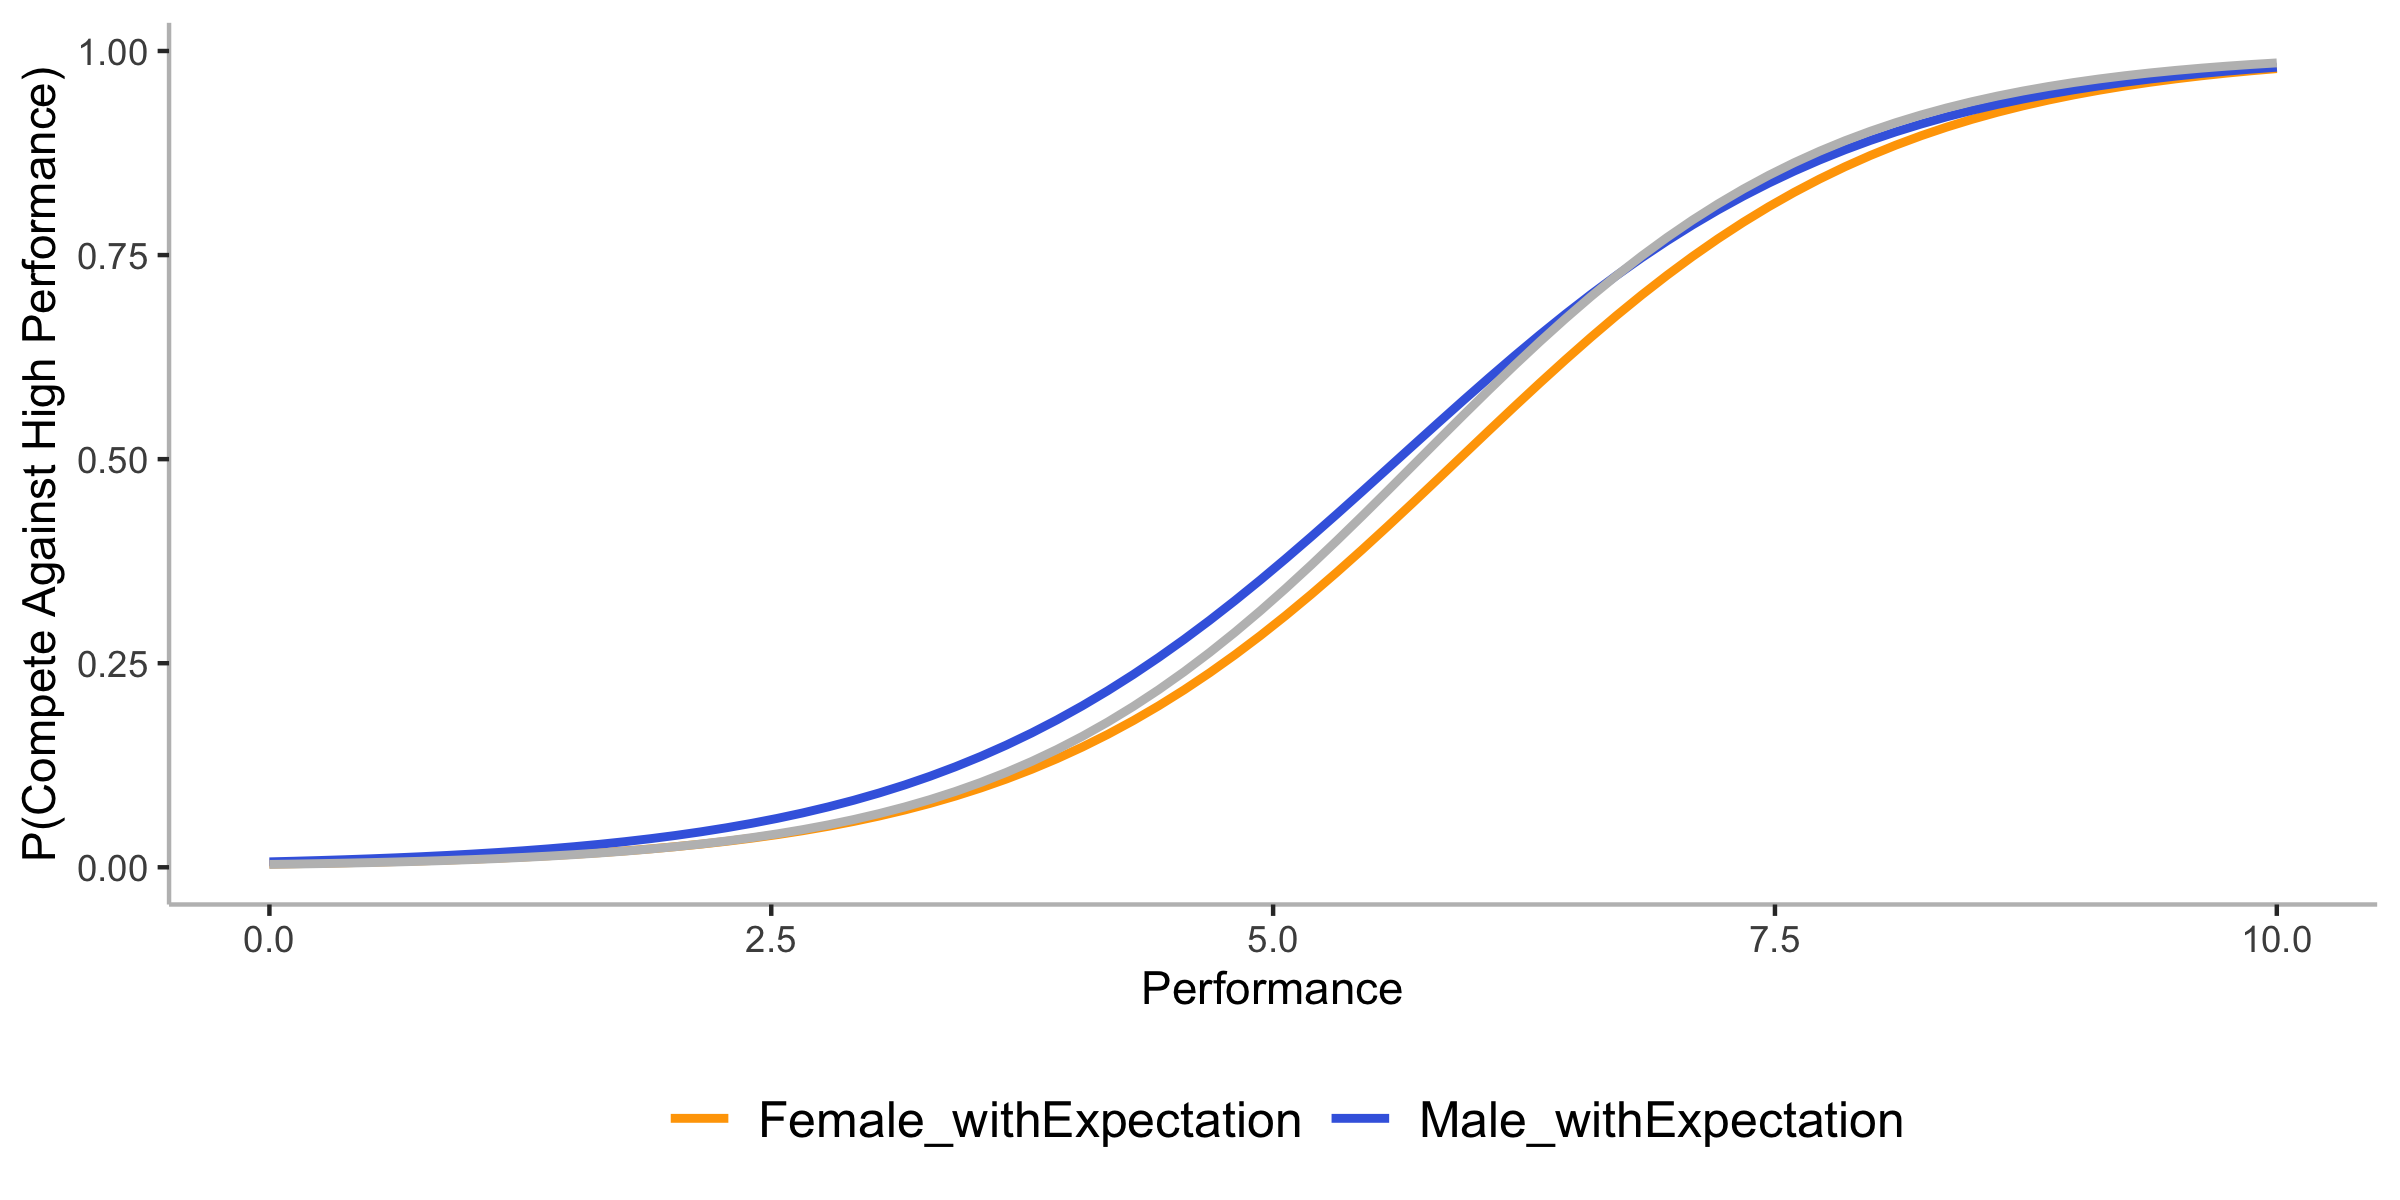
\includegraphics{Advice-Giving_files/figure-latex/study1genderdiff-1} 

}

\caption{Advice given to men and women. Advisers observed real performance and the participants’ estimated performance, but not their gender. As a result of their higher expectations, men were advised to compete against the high performance group more often. In the treatment in which expectations were not shown to the advisors, no gender differences emerged (not displayed in this figure)..}\label{fig:study1genderdiff}
\end{figure}

\begin{figure}

{\centering 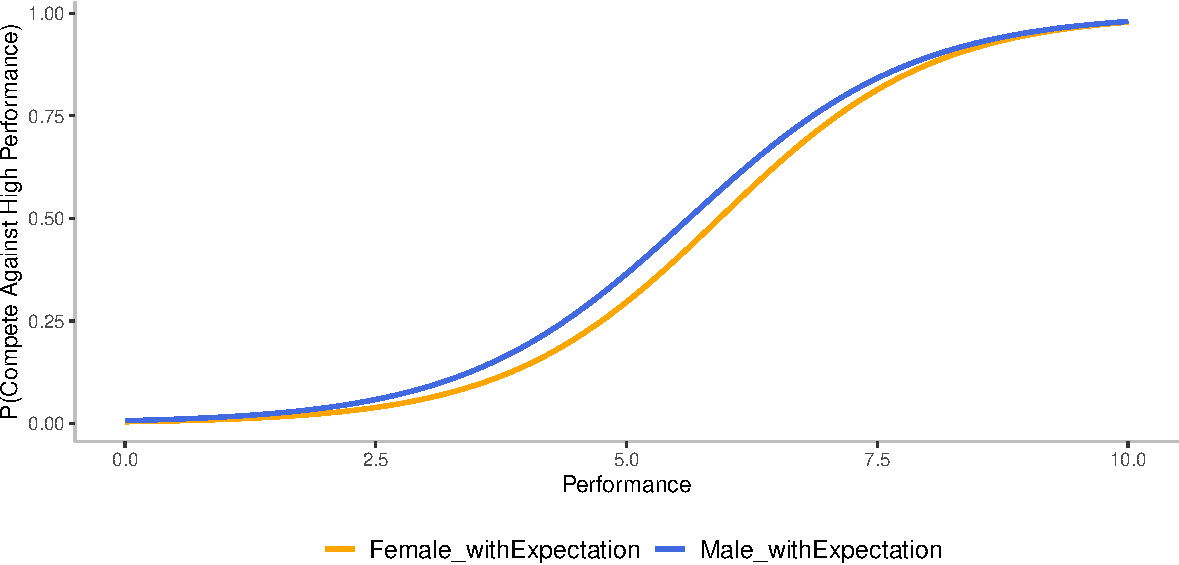
\includegraphics{Advice-Giving_files/figure-latex/unnamed-chunk-3-1} 

}

\caption{ }\label{fig:unnamed-chunk-3}
\end{figure}

Next, we examine whether advisers took the advisee's expectations into account. Column 1 of Table \ref{tab:study1regs} reports a linear probability model on advising to compete against the High Performer group for advisers in the ``Expectations'' treatment. Because each adviser was paired with ten advisees, we cluster standard errors at the adviser level. Consistent with our prediction, we find that advisees in the High Expectation condition are more likely to be recommended to compete against the High Performer Group, but the result is not significant.

To test whether expectations can lead to more flattering advice for men than for women, we report a linear probability model with advice to compete against the high group as the outcome measure, and the advisee's gender, whether expectations were shown to the adviser, and the interaction of the two (Column 2 of Table \ref{tab:study1regs}). As predicted, we find a significant interaction effect: men are more likely to be advised to compete against the High Performers when expectations are shown than when they are hidden (p \textless{} 0.001; see Figure \ref{fig:study1genderdiff},).

To examine the quality of advice, we computed the expected bonus earnings for all recommendations. We made this calculation by assuming that participants adopted the advice and competed against the recommended competitor group. We then compared their scores with all 20 possible competitors one by one and calculated the bonus accordingly to determine the expected bonus earnings. We conducted an OLS regression with whether givers see the expectation (Baseline or Information condition) and the gender of the Advisee (Female or Male), as well as their interaction. Supporting our theory, male participants will receive less bonus given advice they receive (b = -0.005, p \textless{} .01; see also Column 3 of Table \ref{tab:study1regs}

Finally, we look at the actual earnings of advisees. Although participants in the High Expectation condition earned less, this difference is not significant (\(b = -0.02\), 95\% CI \([-0.04, 0.00]\), \(t(948) = -1.92\), \(p = .055\)).

We found that males are more competitive to the extent that they are more likely to choose to compete against High Performer group (\(b = 0.08\), 95\% CI \([0.03, 0.14]\), \(t(948) = 2.89\), \(p = .004\)), holding performance the same.

\hypertarget{discussion}{%
\subsection{Discussion}\label{discussion}}

In Study 1, we discovered that although advisers are encouraged to provide accurate advice, they still take into account the expectations of advisees, which are irrelevant to the utility of the advice. Due to the fact that males tend to be more confident than their equally competent female counterparts, they are more likely to be recommended to compete against high-performance competitors. However, when advice is given to match the advisees' expectations, these flattering recommendations result in lower expected bonus earnings for male participants.

\hypertarget{study-2}{%
\section{Study 2}\label{study-2}}

We then conduct a three-stage experiment to determine why advisers give flattering advice. First, we ask a group of advisees to upload selfies and predict their rank in a group of ten people of the same gender based on physical attractiveness. Next, we recruit and ask advisers to rank selfies of the opposite gender and recommend which rank the participant ranked 7th should bet on, with the bonus being contingent on whether the participant guessed accurately or found the adviser likable. Finally, we show the advisees the advice they have received and ask them to make their final prediction about their rank and evaluate the advice giver in terms of likability, warmth, and trustworthiness. Our main hypothesis is that advisers who want to be liked by advisees would recommend a higher rank.

\hypertarget{methods-1}{%
\subsection{Methods}\label{methods-1}}

We recruited 300 participants and invited them to upload photos of themselves (selfies) to be rated by other participants on attractiveness. We ended up with a sample of 100 men and 107 women who agreed to do so and uploaded usable pictures. We selected the first 100 photos from women to arrive at a gender-balanced sample (\(M_{\text{Age}}\) = 39.37 years; 50.0\% Female). We informed them that their selfies will be randomly grouped into nine others from the same gender and ranked by people of the opposite gender and asked them to predict their rank, with 1st rank represents the most attractive and 10th rank represents the least attractive. We assigned each participant to a group of 10 participants of their own gender.

Next, we recruited 472new participants and asked them to rank the attractiveness of one such group of 10 participants of the opposite gender (\(M_{\text{Age}}\) = 41.03 years; 49.79\% Female). After they did so, we showed them the photo of the participant they ranked as the 7th most attractive (that is, the 4th least attractive) and reminded them that they had ranked this person at 7th attractive. We (truthfully) informed them that this participant would have a chance to earn a bonus if they accurately guessed their rank based on the aggregated ratings of all participants who had ranked this group. Participants were then randomly assigned to an ``accuracy'' or a ``likeability'' treatment. In the accuracy treatment, they were told that they would receive a bonus (\$1) identical to that of the advisee. While in the ``likeability'' treatment, the amount their bonus depended on how the advisee rated them in terms of likeability, after observing only the rank that they had advised the advisee to guess. Advisees would rate to what extent they think the adviser is likable on a 5-point scale, and each point they earn increases their bonus by 20 cents.

Finally, we invited participants from Stage 1 and were ranked as the 7th attractive by at least one adviser (so that they received advice) back for the follow-up survey. Following our preregistration, we kept the survey open for 7 days. In total, 146 participants (77 men, 69 women) returned. They were reminded of the selfie they uploaded in Stage 1 and informed that a group of 10 selfies, including theirs, had been rated by other participants from Prolific. They were also introduced to the opportunity to earn a \$1 bonus if they guessed their rank accurately. Participants were then shown the advice from a randomly selected adviser and made their predictions. After deciding which rank to bet on, advisees were reminded of the advice they received and asked to rate the advice giver's likability, warmth, friendliness, good-naturedness, trustworthiness, and sincerity on a 5-point scale. The last 6 items were adopted from Fiske, Cuddy, and Glick (2007).

\hypertarget{results-1}{%
\subsection{Results}\label{results-1}}

\begin{figure}

{\centering 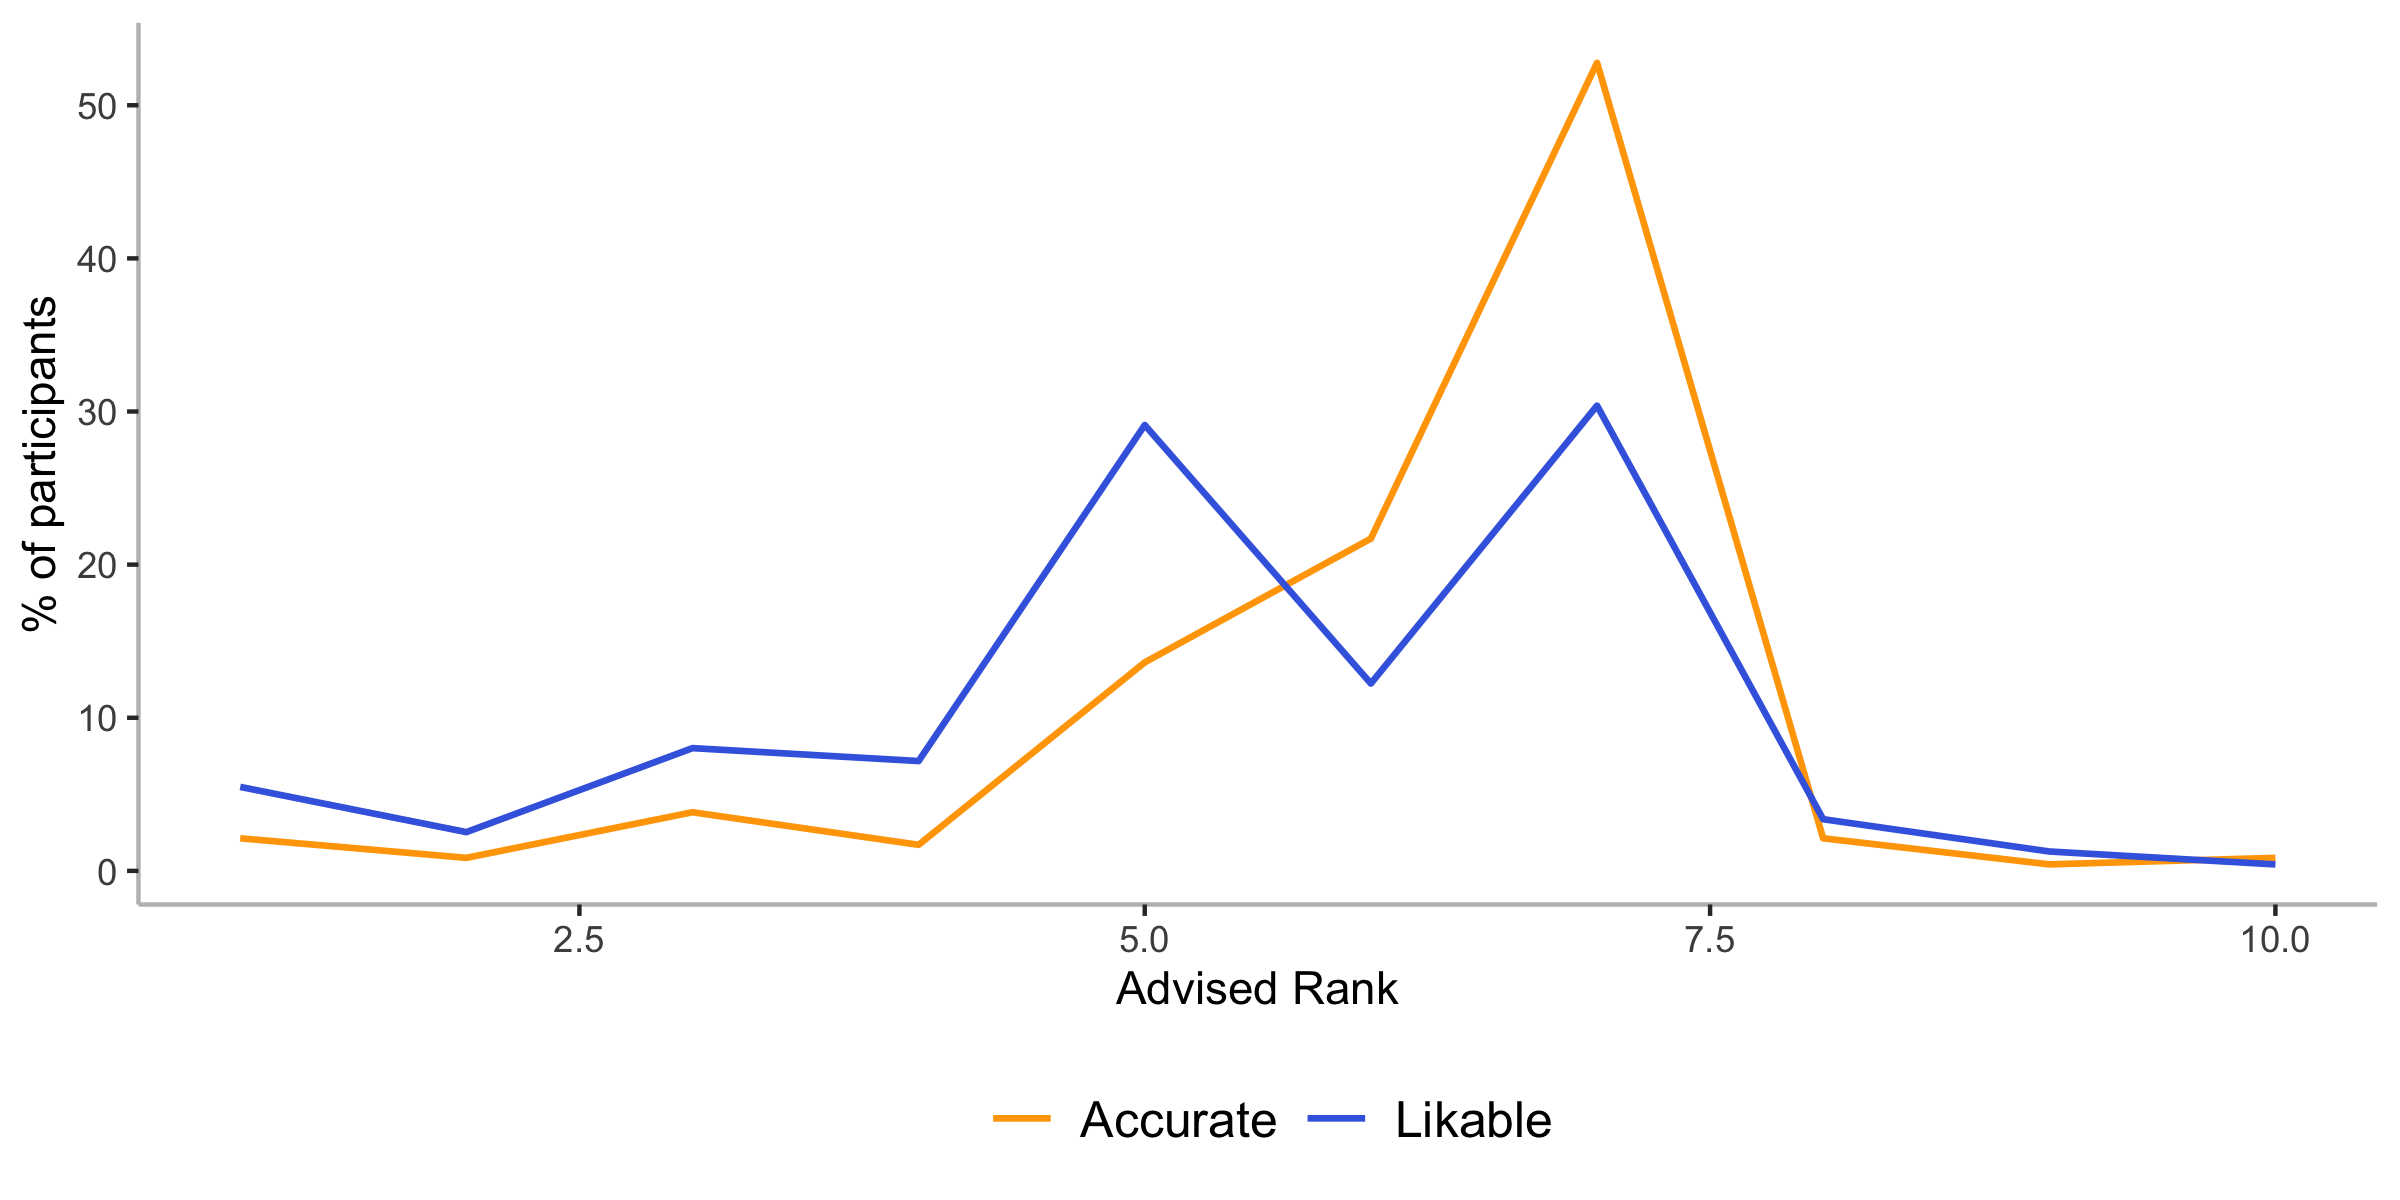
\includegraphics{Advice-Giving_files/figure-latex/study2advice-1} 

}

\caption{Advice for 7th most attractive participants}\label{fig:study2advice}
\end{figure}

Again, we found supportive evidence that males are more confident about themselves, giving higher initial rank prediction (more attractive) than female participants (5.76 vs.~6.37, \(t(205) = 2.15\), \(p = .033\)).

Examining advice from Stage 2 participants, we found that participants advised a lower rank (that is, more attractive) in the likeability treatment than the accuracy treatment (5.38 vs 6.19, \(t(470) = 5.44\), \(p < .001\)). As seen in Figure \ref{fig:study2advice}, notably, however, even in the accuracy treatment, participants advised a lower rank than they themselves had provided (\(t(234) = -8.82\), \(p < .001\)). This suggests that advisers inferred that advising someone that they were more attractive would make the adviser appear more likeable and therefore provided advice that communicated a more favorable impression of the participants' attractiveness.

\begin{table}

\caption{\label{tab:study2regs}When individuals receive advice that implies a high level of attractiveness (lower rank), they tend to perceive the advice giver as more likable (Column 1), warm (Column 2). Column 3 shows that advisors are rated as more trustworthy when they advice lower ranks, but this relationship is only directional.}
\centering
\resizebox{\linewidth}{!}{
\begin{tabular}[t]{lccc}
\toprule
  & (1) & (2) & (3)\\
\midrule
Advised Rank & \num{-0.109}* & \num{-0.133}** & \num{-0.054}\\
 & (\num{0.046}) & (\num{0.044}) & (\num{0.042})\\
Constant & \num{3.777}*** & \num{3.903}*** & \num{3.397}***\\
 & (\num{0.279}) & (\num{0.266}) & (\num{0.257})\\
\midrule
N & \num{146} & \num{146} & \num{146}\\
\bottomrule
\multicolumn{4}{l}{\rule{0pt}{1em}+ p $<$ 0.1, * p $<$ 0.05, ** p $<$ 0.01, *** p $<$ 0.001}\\
\end{tabular}}
\end{table}

\begin{figure}

{\centering 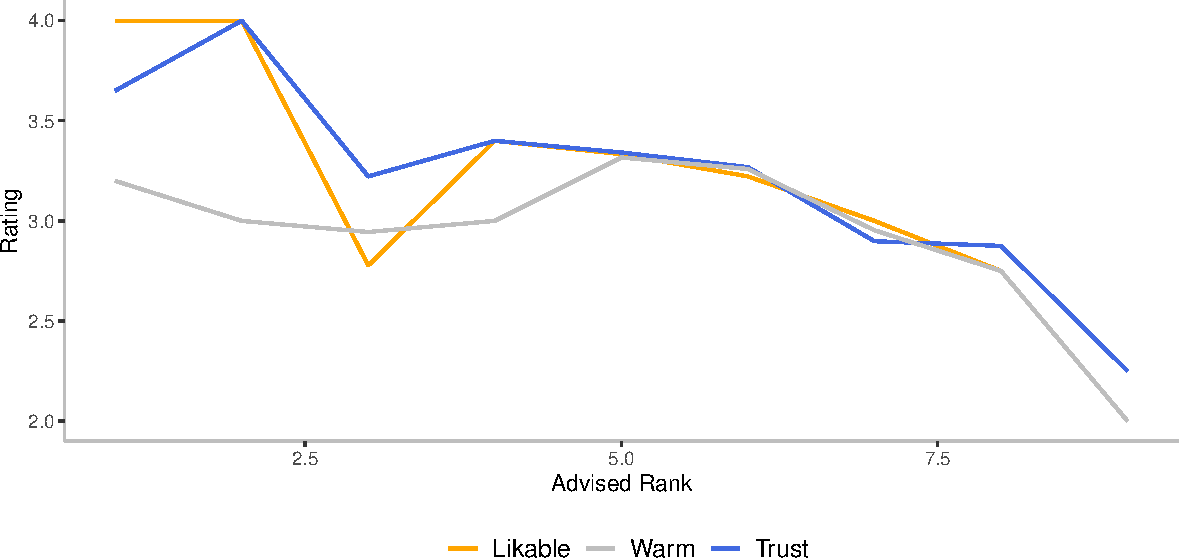
\includegraphics{Advice-Giving_files/figure-latex/study2rating-1} 

}

\caption{The evaluation of advice givers}\label{fig:study2rating}
\end{figure}

To test whether flattering advice brings more positive evaluation of advisers, we create a single index for warmth and trustworthiness by taking average of ratings on warmth, friendliness, good-naturedness, trustworthiness for the former and ratings on trustworthiness, and sincerity for the later. As seen in Figure \ref{fig:study2rating}, we found that advisees who suggested that the advisee was more attractive (lower rank) were indeed rated as more likeable and warm (b = -0.109, p \textless{} .05; b = -0.133, p \textless{} .001; See Columns 1 and 2 of Table 2). Interestingly, these benefits are not at the cost of being hypocritical; advisers are also seen as more trustworthy, but the result is only directional (Column 3 of Table 2). Notably, however, we were not powered to do a comparison across the two experimental groups.

\hypertarget{discussion-1}{%
\section{Discussion}\label{discussion-1}}

dvice substantially shapes people's career and personal outcomes. Therefore, understanding advisers' motivations has far-reaching implications. We propose that advisers' focus on advisees' expectations and the desire to avoid disappointing them can induce gender differences in the advice given and ultimately in the outcomes achieved. Gender differences in career outcomes contribute significantly to the gender wage gap, with women often holding less senior positions and experiencing worse career outcomes, even with equal performance. Therefore, identifying a factor such as expectations that contributes to this gap has important implications for organizational practice.

In this paper, we examine a novel and unexplored factor of advice-giving: interpersonal considerations. Advisers who take into account the advisee's belief utility inflate their advice to convey a more favorable impression, leading to worse decisions and gender differences. Men have more inflated expectations than women, and taking expectations into account can lead to gender differences, even without discrimination. We ruled out discrimination as a separate channel by withholding information about the gender of the advisee. Finally, we expect that advisers are aware of the tradeoff between giving accurate advice and avoiding disappointment and, thus, are less likely to inflate their advice when advisees can compensate them after observing the outcome of their choice.

The findings of this study suggest that organizations can promote gender equity by calibrating employees' expectations or shifting advisers' attention away from them. While these measures may not entirely solve the gender gap problem, they can make a meaningful difference when unconscious bias interventions have failed to show any effect (Chang et al., 2019; Paluck \& Green, 2009). We believe our findings may be particularly relevant to societies that value signaling in interpersonal relationships, including Hong Kong and many Asian countries. Future work could also examine whether people in different cultures place more weight on expectations.

\hypertarget{references}{%
\section{References}\label{references}}

\begingroup
\singlespacing
\setlength{\parindent}{-0.2in}
\setlength{\leftskip}{0.2in}
\noindent

\hypertarget{refs}{}
\begin{CSLReferences}{1}{0}
\leavevmode\vadjust pre{\hypertarget{ref-Ache2020}{}}%
Ache, F., Rader, C., \& Hütter, M. (2020). Advisors want their advice to be used--but not too much: {An} interpersonal perspective on advice taking. \emph{Journal of Experimental Social Psychology}, \emph{89}, 103979.

\leavevmode\vadjust pre{\hypertarget{ref-Benabou2022}{}}%
Bénabou, R., Jaroszewicz, A., \& Loewenstein, G. (2022). \emph{It {Hurts} to {Ask}}. National Bureau of Economic Research.

\leavevmode\vadjust pre{\hypertarget{ref-Benjamin2015}{}}%
Benjamin, D., \& Budescu, D. V. (2015). Advice from experience: {Communicating} incomplete information incompletely. \emph{Journal of Behavioral Decision Making}, \emph{28}(1), 36--49.

\leavevmode\vadjust pre{\hypertarget{ref-Chang2019}{}}%
Chang, E. H., Milkman, K. L., Gromet, D. M., Rebele, R. W., Massey, C., Duckworth, A. L., \& Grant, A. M. (2019). The mixed effects of online diversity training. \emph{Proceedings of the National Academy of Sciences}, \emph{116}(16), 7778--7783.

\leavevmode\vadjust pre{\hypertarget{ref-Exley2022}{}}%
Exley, C., \& Nielsen, K. (2022). The gender gap in confidence: {Expected} but not accounted for. \emph{Available at SSRN 4352381}.

\leavevmode\vadjust pre{\hypertarget{ref-Fiske2007}{}}%
Fiske, S. T., Cuddy, A. J., \& Glick, P. (2007). Universal dimensions of social cognition: Warmth and competence. \emph{Trends in Cognitive Sciences}, \emph{11}(2), 77--83.

\leavevmode\vadjust pre{\hypertarget{ref-Gill2012}{}}%
Gill, D., \& Prowse, V. (2012). A structural analysis of disappointment aversion in a real effort competition. \emph{American Economic Review}, \emph{102}(1), 469--503.

\leavevmode\vadjust pre{\hypertarget{ref-John2019}{}}%
John, L. K., Jeong, M., Gino, F., \& Huang, L. (2019). The self-presentational consequences of upholding one's stance in spite of the evidence. \emph{Organizational Behavior and Human Decision Processes}, \emph{154}, 1--14.

\leavevmode\vadjust pre{\hypertarget{ref-Jonas2003}{}}%
Jonas, E., \& Frey, D. (2003). Information search and presentation in advisor--client interactions. \emph{Organizational Behavior and Human Decision Processes}, \emph{91}(2), 154--168.

\leavevmode\vadjust pre{\hypertarget{ref-Kanze2018}{}}%
Kanze, D., Huang, L., Conley, M. A., \& Higgins, E. T. (2018). We ask men to win and women not to lose: {Closing} the gender gap in startup funding. \emph{Academy of Management Journal}, \emph{61}(2), 586--614.

\leavevmode\vadjust pre{\hypertarget{ref-Koszegi2006}{}}%
Kőszegi, B., \& Rabin, M. (2006). A model of reference-dependent preferences. \emph{The Quarterly Journal of Economics}, \emph{121}(4), 1133--1165.

\leavevmode\vadjust pre{\hypertarget{ref-Kray2000}{}}%
Kray, L. J. (2000). Contingent weighting in self-other decision making. \emph{Organizational Behavior and Human Decision Processes}, \emph{83}(1), 82--106.

\leavevmode\vadjust pre{\hypertarget{ref-Kray1999}{}}%
Kray, L., \& Gonzalez, R. (1999). Differential weighting in choice versus advice: {I}'ll do this, you do that. \emph{Journal of Behavioral Decision Making}, \emph{12}(3), 207--218.

\leavevmode\vadjust pre{\hypertarget{ref-Loewenstein1987}{}}%
Loewenstein, G. (1987). Anticipation and the valuation of delayed consumption. \emph{The Economic Journal}, \emph{97}(387), 666--684.

\leavevmode\vadjust pre{\hypertarget{ref-Loewenstein2018}{}}%
Loewenstein, G., \& Molnar, A. (2018). The renaissance of belief-based utility in economics. \emph{Nature Human Behaviour}, \emph{2}(3), 166--167.

\leavevmode\vadjust pre{\hypertarget{ref-Paluck2009}{}}%
Paluck, E. L., \& Green, D. P. (2009). Prejudice reduction: What works? A review and assessment of research and practice. \emph{Annual Review of Psychology}, \emph{60}, 339--367.

\leavevmode\vadjust pre{\hypertarget{ref-Shalvi2019}{}}%
Shalvi, S., Soraperra, I., Weele, J. J. van der, \& Villeval, M. C. (2019). \emph{Shooting the messenger? Supply and demand in markets for willful ignorance}.

\end{CSLReferences}

\endgroup


\end{document}
